\documentclass[a4paper,oneside, 10pt]{article}

\usepackage[english]{babel}
\usepackage[T1]{fontenc}
\usepackage[utf8]{inputenc}
\usepackage{amsmath}

\usepackage{ltxtable, longtable}
\usepackage{rotating}

\usepackage{graphicx}
\usepackage{pifont}
\usepackage{hyperref}
\usepackage{fancyref}
\usepackage{tabularx}
\usepackage{tabulary}
\usepackage[margin=1cm]{caption}
\usepackage{listings}
\usepackage[section]{placeins}
\usepackage{fancyhdr}
\usepackage[yyyymmdd]{datetime}

\usepackage{morefloats}
\usepackage{tikz}
\usetikzlibrary{shapes, arrows}






\lstdefinestyle{customc}{
  belowcaptionskip=1\baselineskip,
  breaklines=true,
  frame=L,
  xleftmargin=\parindent,
  language=C,
  showstringspaces=false,
  basicstyle=\footnotesize\ttfamily,
  keywordstyle=\bfseries\color{green!40!black},
  commentstyle=\itshape\color{purple!40!black},
  identifierstyle=\color{blue},
  stringstyle=\color{orange},
}

\lstdefinestyle{customsh}{
  belowcaptionskip=1\baselineskip,
  breaklines=true,
  frame=L,
  xleftmargin=\parindent,
  language=C,
  showstringspaces=false,
  basicstyle=\footnotesize\ttfamily,
  keywordstyle=\bfseries\color{green!40!black},
  commentstyle=\itshape\color{purple!40!black},
  identifierstyle=\color{blue},
  stringstyle=\color{orange},
}
\title{Genomizer}
\def\version{2.4}

\def\json{\texttt{JSON}}
\renewcommand{\fullref}[1]{\autoref{#1} on page \pageref{#1}}

\renewcommand{\nomlabel}[1]{\textbf{\titlecap{#1}}}

\newcommand{\appName}{\textit{Genomizer}}
\newcommand{\addImage}[1]{\centering\includegraphics[width=\textwidth, keepaspectratio=true]{#1}}
\newcommand{\addScaledImage}[2]{\centering\includegraphics[width=#1\textwidth]{#2}}
\newcommand{\addImageVertical}[1]{\centering\includegraphics[height=\textwidth, angle=90, keepaspectratio=true]{#1}}
\newcommand{\addScaledImageVertical}[2]{\centering\includegraphics[scale=#1, angle=90]{#2}}
\newcommand{\refer}[1]{\autoref{#1}}
\newcommand{\addCode}[3][c]{\lstinputlisting[caption=#3, escapechar=, style=custom#1]{#2}}
\newcommand{\filePath}[1]{\texttt{#1}}
%\newcommand{\click}[1]{\ding{43} \textbf{\textit{{#1}}}}
\newcommand{\click}[1]{\textbf{\textit{{#1}}}}
\newcommand{\term}[1]{\textit{#1}}
\newcommand{\strongTerm}[1]{\textbf{\term{#1}}}
\newcommand{\serverPort}{\texttt{7000}}
\newcommand{\class}[1]{\texttt{#1}}

\newcommand{\userstory}[2]{
\begin{tabularx}{0.95\textwidth}{|X|}
\hline
\vspace{1pt}
\large\textbf{#1} \\ 
\hline
\vspace{1pt}
#2 \\
\hline
\end{tabularx}
}

\newcommand{\addTwoImages}[4]{
\centering
\begin{tabular}{l l}
    \begin{minipage}{0.4\textwidth}
        
        \includegraphics[width=\textwidth, keepaspectratio=true]{#1} 
	\caption*{#2}

    \end{minipage}
& 
    \begin{minipage}{0.4\textwidth}
        
        \includegraphics[width=\textwidth, keepaspectratio=true]{#3} 
	\caption*{#4}

    \end{minipage}
\\ 
\end{tabular}
}

\fancypagestyle{preface}
{
	\fancyhead[L]{PREFACE}
	\fancyhead[R]{\thepage}

}


\newcommand{\addThreeImages}[6]{
\centering
\begin{tabular}{l l l}
    \begin{minipage}{0.3\textwidth}

        \includegraphics[width=\textwidth, keepaspectratio=true]{#1} 
	\caption*{#2}

    \end{minipage}
& 
    \begin{minipage}{0.3\textwidth}

        \includegraphics[width=\textwidth, keepaspectratio=true]{#3} 
	\caption*{#4}

    \end{minipage}
&
    
    \begin{minipage}{0.3\textwidth}

        \includegraphics[width=\textwidth, keepaspectratio=true]{#5} 
	\caption*{#6}

    \end{minipage}
\\ 
\end{tabular}
}

\newcommand{\addFourImages}[8]{
\centering
\begin{tabular}{l l}
    \begin{minipage}{0.4\textwidth}
        
        \includegraphics[width=\textwidth, keepaspectratio=true]{#1} 
	\caption*{#2}

    \end{minipage}
& 
    \begin{minipage}{0.4\textwidth}
        
        \includegraphics[width=\textwidth, keepaspectratio=true]{#3} 
	\caption*{#4}

    \end{minipage}
\\ 
    \begin{minipage}{0.4\textwidth}
        
        \includegraphics[width=\textwidth, keepaspectratio=true]{#5} 
	\caption*{#6}

    \end{minipage}
&
    \begin{minipage}{0.4\textwidth}
        
        \includegraphics[width=\textwidth, keepaspectratio=true]{#7} 
	\caption*{#8}

    \end{minipage}
\\
\end{tabular}
}

\setcounter{secnumdepth}{5}

\setlength{\parindent}{0pt}
\setlength{\parskip}{10pt}

\graphicspath{ {figures/}}



\usepackage{lmodern}
\usepackage{fixltx2e} % provides \textsubscript
% use upquote if available, for straight quotes in verbatim environments
\IfFileExists{upquote.sty}{\usepackage{upquote}}{}
% use microtype if available
\IfFileExists{microtype.sty}{%
\usepackage{microtype}
\UseMicrotypeSet[protrusion]{basicmath} % disable protrusion for tt fonts
}{}
\usepackage{color}
\usepackage{fancyvrb}
\newcommand{\VerbBar}{|}
\newcommand{\VERB}{\Verb[commandchars=\\\{\}]}
\DefineVerbatimEnvironment{Highlighting}{Verbatim}{commandchars=\\\{\}}
% Add ',fontsize=\small' for more characters per line
\newenvironment{Shaded}{}{}
\newcommand{\KeywordTok}[1]{\textcolor[rgb]{0.00,0.44,0.13}{\textbf{{#1}}}}
\newcommand{\DataTypeTok}[1]{\textcolor[rgb]{0.56,0.13,0.00}{{#1}}}
\newcommand{\DecValTok}[1]{\textcolor[rgb]{0.25,0.63,0.44}{{#1}}}
\newcommand{\BaseNTok}[1]{\textcolor[rgb]{0.25,0.63,0.44}{{#1}}}
\newcommand{\FloatTok}[1]{\textcolor[rgb]{0.25,0.63,0.44}{{#1}}}
\newcommand{\CharTok}[1]{\textcolor[rgb]{0.25,0.44,0.63}{{#1}}}
\newcommand{\StringTok}[1]{\textcolor[rgb]{0.25,0.44,0.63}{{#1}}}
\newcommand{\CommentTok}[1]{\textcolor[rgb]{0.38,0.63,0.69}{\textit{{#1}}}}
\newcommand{\OtherTok}[1]{\textcolor[rgb]{0.00,0.44,0.13}{{#1}}}
\newcommand{\AlertTok}[1]{\textcolor[rgb]{1.00,0.00,0.00}{\textbf{{#1}}}}
\newcommand{\FunctionTok}[1]{\textcolor[rgb]{0.02,0.16,0.49}{{#1}}}
\newcommand{\RegionMarkerTok}[1]{{#1}}
\newcommand{\ErrorTok}[1]{\textcolor[rgb]{1.00,0.00,0.00}{\textbf{{#1}}}}
\newcommand{\NormalTok}[1]{{#1}}
\usepackage{graphicx}
\makeatletter
\def\maxwidth{\ifdim\Gin@nat@width>\linewidth\linewidth\else\Gin@nat@width\fi}
\def\maxheight{\ifdim\Gin@nat@height>\textheight\textheight\else\Gin@nat@height\fi}
\makeatother
% Scale images if necessary, so that they will not overflow the page
% margins by default, and it is still possible to overwrite the defaults
% using explicit options in \includegraphics[width, height, ...]{}
\setkeys{Gin}{width=\maxwidth,height=\maxheight,keepaspectratio}
\ifxetex
  \usepackage[setpagesize=false, % page size defined by xetex
              unicode=false, % unicode breaks when used with xetex
              xetex]{hyperref}
\else
%  \usepackage[unicode=true]{hyperref}
\fi


\begin{document}
\makeatletter
\renewcommand\paragraph{%
   \@startsection{paragraph}{4}{0mm}%
      {-\baselineskip}%
      {.5\baselineskip}%
      {\normalfont\normalsize\bfseries}}

\renewcommand\subparagraph{%
   \@startsection{paragraph}{4}{0mm}%
      {-\baselineskip}%
      {.5\baselineskip}%
      {\normalfont\normalsize\bfseries}}
 
 \renewcommand\subsection{%
   \@startsection{subsection}{4}{0mm}%
      {-\baselineskip}%
      {.5\baselineskip}%
      {\normalfont\normalsize\bfseries}}
\makeatother



\pagestyle{fancy}

\appName\ is a system for storing and analyzing \term{DNA}-sequence data. It was designed for researchers in the field of epigenetics, who are interested in where on a \term{DNA} string certain proteins binds. In order to get this information, experiments are conducted and \term{raw} data files collected. These data files are then converted, in a series of steps, to files suitable for analysis. These files are hence refered to as \term{profile} data. \appName\ allows the researchers to upload \term{raw} files to a server and automate the generation of analysis data aswell as store the generated analysis data in a database for later access. 

The documentation contains three main parts. Introduction chapters that explain the goal of the project aswell as a non-technical description of the project implementation. The development part of the document where the current implementation of each part of the project is explained how they look and work aswell as an attempt to explain why certain design choices where done. Then finally there is a big collection of appendicies that goes deeper in their explenation of certain details of the implementation aswell as maintenance guides.

\nomenclature{raw}{Collection word for files that are the result from a \textit{DNA}-sequencing machine.}
\nomenclature{profile}{Data converted to a human readable file for analysis.}

The \appName\ system was designed with a specific target group in mind: Epigenitic researchers. This chapter will explain the needs of these users, the problems they faced before this system was provided and the requirements that were collected and taken into account during the project.
\nomenclature{Genomizer}{Collective name for the project.}
\section{Target group}

The target group for the \appName\ system is  \term{Epigenetic Cooperation Norrland (EpiCoN)}, a diverse group of researchers at \term{Umeå University} made up of many different nationalities. Their main communication language is English.

\term{EpiCon} are involved in the research of how proteins bind to \term{DNA} strings and its effects. Experiments are carried out which yield large amounts of raw data. This information, combined with knowledge about the location of genes within a given genome, enable the researchers to gain valuable information about which proteins are active in enabling and disabling genes. These results are important in the study of how cells ''remember'' which genes should be enabled after cell division.

Previous to the \appName\ project the raw data files retrieved from experiments were manually processed by the researchers using inefficient \term{Perl} scripts. This process also involved using \term{Bowtie}\cite{BOWTIE}, a program used to unscramble the \term{DNA} data, and \term{LiftOver}\cite{LIFTOVER} which is used to adjust results to conform to different \term{genome releases}.

The researchers at \term{EpiCoN} have varying computer skills. While they all have basic computer knowledge, not all are familiar with more advanced computing tasks such as running scripts at command line level. As such, some researchers have become dependent on others to process the raw data. At \term{EpiCon} the researcher that has the knowledge to use all the scripts and software performs many of these time consuming tasks for other researchers.

From time to time students of molecular biology are interested in working with the data, however their access is limited to viewing and analysing the data. 

\nomenclature{Bowtie}{Program the preforms parsing of the raw data and counts base pairs}
\nomenclature{liftOver}{Converts genome release versions.}
\nomenclature{genome releases}{Constant research gives more understanding, new genome versions are often found.}

\section{Client needs}
The researchers at \term{EpiCoN} need a system to structure the large amount of genetic data they use daily. The requirements, as described below, were collected and handled as a number of \term{user stories}, each of which describe a desired function from the end users perspective. A complete list of the \term{user stories} are presented in \fullref{chap:userstories}. %When discussed below the title of the relevant \term{user story} will be used.
A overview of the requested system may be seen below in \refer{fig:requestOverview}. Where orange colored nodes are must have features while gray nodes are visions of the clients that may be implemented if time allows for it.

There are three main data types used in the research and that the system should handle: \term{raw}, \term{profile} and \term{region} data. \term{Raw} data is the raw output from an experiment and cannot be analysed directly. It is first processed to so called \term{profile} data. \term{Profile} data describes the amount of reads found for every base--pair in an organism's genome. \term{Region} data is further processed \term{profile} data consisting of the regions where every base--pair's read strength is above a given threshold and fault tolerance. The region gets a value based on the average of the base-pair reads for the given region.

\nomenclature{region}{Region data is small parts of the profile data.}
\begin{figure}[h!]
\centering
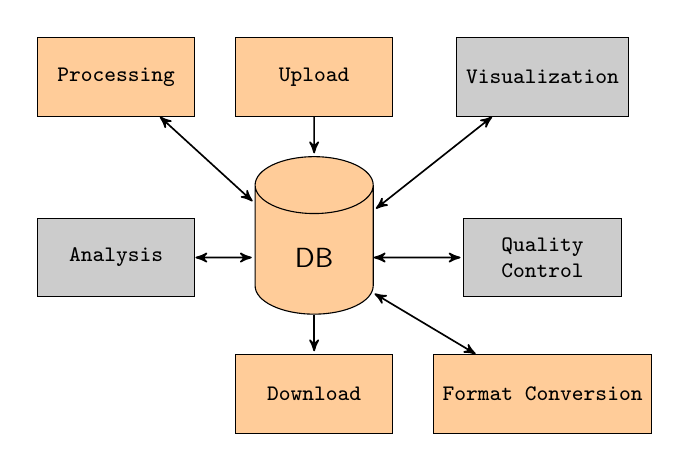
\begin{tikzpicture}[ 
	font=\sffamily,
  every matrix/.style={ampersand replacement=\&,column sep=0.5cm,row sep=0.5cm},
  db/.style={cylinder, shape border rotate=90, draw, fill=orange!40, minimum height=2cm, minimum width=1.5cm},
  must/.style={rectangle, draw, fill=orange!40, minimum height=1cm, minimum width=2cm, font=\ttfamily\footnotesize},
  vision/.style={rectangle, draw, fill=gray!40, minimum height=1cm, minimum width=2cm, font=\ttfamily\footnotesize}, 
  both/.style={<->,>=stealth',shorten >=1pt,semithick,font=\sffamily\footnotesize},
  to/.style={->,>=stealth',shorten >=1pt,semithick,font=\sffamily\footnotesize},
  every node/.style={align=center}]
  
\matrix{
	\node[must] (proc) {Processing}; \&
	\node[must] (add) {Upload}; \&
	\node[vision] (visual) {Visualization}; \\
	\node[vision] (analys) {Analysis}; \& 
	\node[db] (B) {DB}; \& 
	\node[vision] (quality) {Quality\\ Control}; \\
 	\& 	\node[must] (extract) {Download}; \&
 	\node[must] (format) {Format Conversion}; \\
	};
	
	\draw[both] (proc) -- (B);
	\draw[to] (add) -- (B);
	\draw[both] (visual) -- (B);
	\draw[both] (analys) -- (B);
	\draw[both] (B) -- (quality);
	\draw[to] (B) -- (extract);	
	\draw[both] (format) -- (B);

\end{tikzpicture}
\caption{\footnotesize Overview of targeted system}
\label{fig:requestOverview}
\end{figure}

\subsection{Upload \& Download}

When conducting experiments the researchers generate \term{raw} data that generates what they call \term{Raw}-files. These files along with profile data, region data and genome release data may be added and related to an experiment. The requested functionality is to be able to upload these files to the database from multiple sources. The sources may be directly from an experiment conducted by the researchers or from official publications.

When results are published in scientific articles the \term{raw} data from the experiments are often also provided. One location where these \term{raw} data files can be published is the \term{GEO} (\term{Gene Expression Omnibus}) database. A desire to be able to initialize an upload to \appName\ with the source of the upload beeing  \term{GEO}.

\nomenclature{GEO}{Centralized database where article data can be found.}

\subsection{Database}
The \texttt{Database} module requested has the purpose to archive experiment data in a way of easy access. To allow for this the experiments and files associated with them needs to have information vital for good readability. This is solved with the help of annotations. The researchers must add annotations to files related to an experiment.
This data is the foundation for further research and so must be stored securely. To ensure security the client requested a system for authorization that protects the data from outside tampering. To protect against hardware failure there exists a request for a backup system.

\subsection{Processing}
The unordered \term{raw} data gained from an experiment requires processing in order to be analysed. The researchers have written a number of scripts and, when combined with the \term{BowTie} algorithm, generate \term{profile} data. In this format the \term{DNA} pieces are ordered and mapped to the \term{DNA} string. It is important that the system automates this process so that all researchers can easily process the large \term{raw} files.

As new discoveries are made in the area, new standards for the order of the base pairs in a \term{DNA} string are set. This results in a new \term{Genome Release} for a specific species. These are obtained as a set of files specifying this order and are used in the processing of \term{raw} data. \appName\ must support the uploading of new sets of \term{genome release} files to be used in processing otherwise the system will very quickly become outdated. 

It would also be an advantage if the system could carry out further processing from \term{profile} to \term{region} files.

After processing, the resulting data files should be annotated and saved in the database alongside their parent files. It is important that the parent files remain traceable and that the parameters used in processing are saved so that the process can be repeated and confirmed.

\subsection{Format Conversion}
\appName\ should also provide a way to convert \term{profile} data files between different genome releases. This involves the ability to upload new \term{Chain Files} which enable conversion using \term{LiftOver} and the embedding of this program. The \term{LiftOver} program compares the differences between two genome releases and converts it to one update genome release.

It is not uncommon to discover errors in a new release after publication, thus it is important to store files generated using older genome releases, even though newer releases has been published to allow for \term{LiftOver} conversion.

\nomenclature{Chain files}{Genome release files with small alterations to previous genome releases.}





This chapter will present an overview of the services that the \appName\ system currently provides. 

\section{Usage}



\begin{figure}[h]
\addImage{genomizerDiagramServiceDescription.png}
\caption{Communication diagram of the product}
\label{fig:con_serviceDescription}
\end{figure}
	
In order to give the users flexibility when using the service there are clients for many different platforms (Windows, Linux, OSX, Web, Mobile devices). 
When a user chooses a given task, for example start \term{raw} to \term{profile} processing, that task is sent via Internet to the server as shown in \refer{fig:con_serviceDescription} which will handle the request and send a response back to the user.

\section{User Input}
The user input in the \appName/ system may be done with four different clients: a desktop client, a web client, an \textit{Android} client and a \textit{iOS} client. The last two clients are collected under mobile application since they offer the same functionality.

\section{Desktop}
The desktop client is the main client for the \appName system. It offers all implemented functionality. 
\begin{itemize}
\item Login and logout.
\item Searching for experiments and different files.
\item Create new experiments.
\item Modify existing experiments.
\item Upload files to experiments.
\item Download files from experiments.
\item Process files from raw to profile.
\item Delete files and experiments from the database.
\item Add annotations to experiments.
\item Remove and modify annotations.
\item Search annotations by name.
\item Upload, remove and rename genome release files.
\end{itemize}

\section{Web}
The web client mimics the behaviour and functionality of the desktop client. Additionally, unlike the desktop client, it enables the user to log in and use the service remotely via Internet. This is useful if the user needs to, for example, download or upload files to the server but is not currently on the same local network as the server. The web client is easy to start using since it runs in a web browser and needs no installation.


\section{Mobile application}
Due to the limited storage available on mobile devices it is not appropriate to enable uploading and downloading of files, however the mobile applications enable the searching of files in the database and the scheduling of processing procedures for the conversion of \term{raw} to \term{profile} data.

\section{Server}
The servers purpose is to take care of the organizations of files and experiments as seen in the top part of Figure \ref{fig:con_serviceDescription} as the part \textit{Data storage}. The server also has the purpose of taking care of the heavy workload of processing the files added to the \textit{Data storage}.

\subsection{Data storage}
The main purpose of the \appName\ system is to centralize all data. To enable this a user can annotate and upload data to the server using both desktop and web based clients.
Advanced database searches can be performed on the annotations to find previously uploaded data. When the required data is found the user can choose to download the files or request that they be processed on the server.
\subsubsection{Experiments}


\subsubsection{Annotations}
Annotations is a way for the researchers to keep track of what an experiment consists of aswell as files associated with an experiment.
\appName has two kinds of annotations. There is \textit{multiple-choice} annotations which have a defined name and choices. An example is the annotation named \textit{species} that have the choices human, fly and rat.
Then there is \textit{free text} annotations where the user may enter what they want.

Dynamic annotations must also be managed in order to keep the system clean and up to date. \appName\ therefore provides full editing options for existing annotations if the user have the credentials. This includes the editing of \term{mulitple-choice} annotation choices and the removal of unused annotations.

\begin{example}
If the user has an experiment that was conducted in zero gravity and the database does not have the annotation field ``Zero Gravity'' the user can add this as a new annotation. In this case a \term{Drop Down} annotation type may be appropriate, with the simple choices ``yes'' or ``no''. Of course it is also possible to leave the annotation type as \term{Free Text} which enables users to write  freely the value of the annotation.
\end{example}

\subsection{Processing}
Users can request that a \term{raw} file set be processed to \term{profile} files. This procedure is carried out on the server to avoid heavy workload and the requirements of certain programs on the clients side. The processing carried out between \term{raw} data and \term{profile} data involves a number of different steps. The user can choose which steps are carried out and the various parameters used.



\end{document}
